\documentclass{article}
\usepackage{amsmath}
\usepackage[latin1,utf8]{inputenc}
\usepackage{tikz}
\usetikzlibrary{arrows}
\usetikzlibrary{arrows.meta}
\usetikzlibrary{positioning, shapes.arrows, backgrounds}
\usepackage{xcolor}

\newcommand{\deletionElement}{\alpha}

\begin{document}

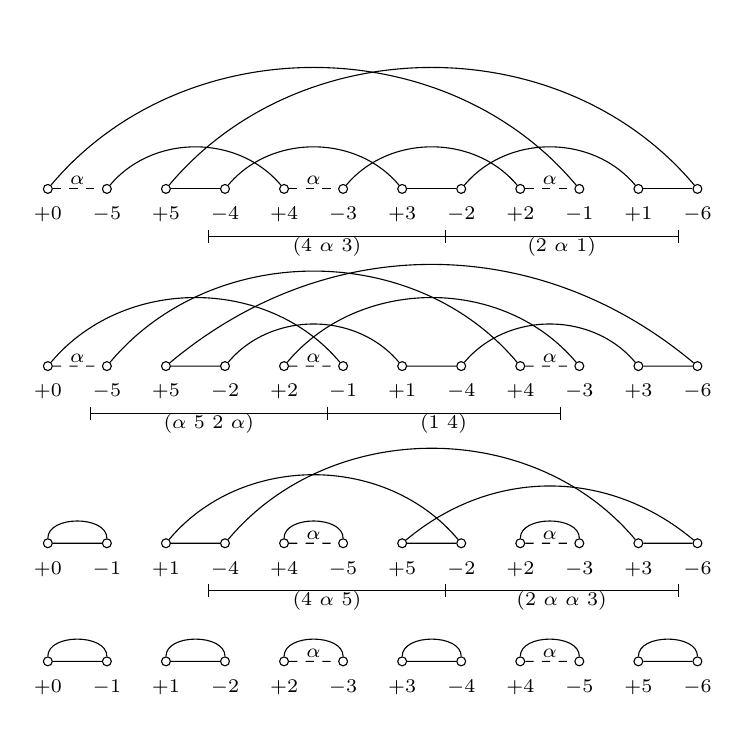
\begin{tikzpicture}[scale=0.75]
\scriptsize
\begin{scope}[every node/.style={inner sep=0.4mm, draw, circle, minimum size = 0pt}]
    \node[label=below:$+0$] (p0) at (0,0) {};
    \node[label=below:$-5$] (m5) at (1,0) {};
    \node[label=below:$+5$] (p5) at (2,0) {};
    \node[label=below:$-4$] (m4) at (3,0) {};
    \node[label=below:$+4$] (p4) at (4,0) {};
    \node[label=below:$-3$] (m3) at (5,0) {};
    \node[label=below:$+3$] (p3) at (6,0) {};
    \node[label=below:$-2$] (m2) at (7,0) {};
    \node[label=below:$+2$] (p2) at (8,0) {};
    \node[label=below:$-1$] (m1) at (9,0) {};
    \node[label=below:$+1$] (p1) at (10,0) {};
    \node[label=below:$-6$] (m6) at (11,0) {};
\end{scope}

\begin{scope}[dashed]
    \path [-] (p0) edge node [black, pos=0.5, sloped, above, yshift=-0.05cm] {$\deletionElement$} (m5);
    \path [-] (p4) edge node [black, pos=0.5, sloped, above, yshift=-0.05cm] {$\deletionElement$} (m3);
    \path [-] (p2) edge node [black, pos=0.5, sloped, above, yshift=-0.05cm] {$\deletionElement$} (m1);
\end{scope}

\begin{scope}[every edge/.style={draw=black}]
    \path [-] (p5) edge node [black, pos=0.5, sloped, above, yshift=-0.05cm] {} (m4);
    \path [-] (p3) edge node [black, pos=0.5, sloped, above, yshift=-0.05cm] {} (m2);
    \path [-] (p1) edge node [black, pos=0.5, sloped, above, yshift=-0.05cm] {} (m6);
\end{scope}

\begin{scope}[every edge/.style={draw=black}]
    \path [-] (p0) edge  [bend left=50] (m1);
    \path [-] (p1) edge  [bend right=50] (m2);
    \path [-] (p2) edge  [bend right=50] (m3);
    \path [-] (p3) edge  [bend right=50] (m4);
    \path [-] (p4) edge  [bend right=50] (m5);
    \path [-] (p5) edge  [bend left=50] (m6);
\end{scope}

\begin{scope}[every edge/.style={draw=black}, every node/.style={inner sep=0pt, minimum size = 0pt}]
\node[label=\phantom{}] (bi1) at (2.7, -0.8) {};
\node[label=\phantom{}] (bi2) at (6.75, -0.8) {};
\path [{Bar}-{Bar}] (bi1) edge node [black, pos=0.5, sloped, below] {$(4~\deletionElement~3)$} (bi2);

\node[label=\phantom{}] (bi3) at (6.7, -0.8) {};
\node[label=\phantom{}] (bi4) at (10.7, -0.8) {};
\path [-{Bar}] (bi3) edge node [black, pos=0.5, sloped, below] {$(2~\deletionElement~1)$} (bi4);
\end{scope}


\begin{scope}[every node/.style={inner sep=0.4mm, draw, circle, minimum size = 0pt}]
    \node[label=below:$+0$] (2p0) at (0,-3) {};
    \node[label=below:$-5$] (2m5) at (1,-3) {};
    \node[label=below:$+5$] (2p5) at (2,-3) {};
    \node[label=below:$-2$] (2m2) at (3,-3) {};
    \node[label=below:$+2$] (2p2) at (4,-3) {};
    \node[label=below:$-1$] (2m1) at (5,-3) {};
    \node[label=below:$+1$] (2p1) at (6,-3) {};
    \node[label=below:$-4$] (2m4) at (7,-3) {};
    \node[label=below:$+4$] (2p4) at (8,-3) {};
    \node[label=below:$-3$] (2m3) at (9,-3) {};
    \node[label=below:$+3$] (2p3) at (10,-3) {};
    \node[label=below:$-6$] (2m6) at (11,-3) {};
\end{scope}

\begin{scope}[dashed]
    \path [-] (2p0) edge node [black, pos=0.5, sloped, above, yshift=-0.05cm] {$\deletionElement$} (2m5);
    \path [-] (2p2) edge node [black, pos=0.5, sloped, above, yshift=-0.05cm] {$\deletionElement$} (2m1);
    \path [-] (2p4) edge node [black, pos=0.5, sloped, above, yshift=-0.05cm] {$\deletionElement$} (2m3);
\end{scope}

\begin{scope}[every edge/.style={draw=black}]
    \path [-] (2p5) edge node [black, pos=0.5, sloped, above, yshift=-0.05cm] {} (2m2);
    \path [-] (2p1) edge node [black, pos=0.5, sloped, above, yshift=-0.05cm] {} (2m4);
    \path [-] (2p3) edge node [black, pos=0.5, sloped, above, yshift=-0.05cm] {} (2m6);
\end{scope}


\begin{scope}[every edge/.style={draw=black}]
\end{scope}

\begin{scope}[every edge/.style={draw=black}]
    \path [-] (2p0) edge  [bend left=50] (2m1);
    \path [-] (2p1) edge  [bend right=50] (2m2);
    \path [-] (2p2) edge  [bend left=50] (2m3);
    \path [-] (2p3) edge  [bend right=50] (2m4);
    \path [-] (2p4) edge  [bend right=50] (2m5);
    \path [-] (2p5) edge  [bend left=40] (2m6);
\end{scope}

\begin{scope}[every edge/.style={draw=black}, every node/.style={inner sep=0pt, minimum size = 0pt}]
\node[label=\phantom{}] (bi1) at (0.7, -3.8) {};
\node[label=\phantom{}] (bi2) at (4.75, -3.8) {};
\path [{Bar}-{Bar}] (bi1) edge node [black, pos=0.5, sloped, below] {$(\deletionElement~5~2~\deletionElement)$} (bi2);

\node[label=\phantom{}] (bi3) at (4.7, -3.8) {};
\node[label=\phantom{}] (bi4) at (8.7, -3.8) {};
\path [-{Bar}] (bi3) edge node [black, pos=0.5, sloped, below] {$(1~4)$} (bi4);
\end{scope}

\begin{scope}[every node/.style={inner sep=0.4mm, draw, circle, minimum size = 0pt}]
    \node[label=below:$+0$] (3p0) at (0,-6) {};
    \node[label=below:$-1$] (3m1) at (1,-6) {};
    \node[label=below:$+1$] (3p1) at (2,-6) {};
    \node[label=below:$-4$] (3m4) at (3,-6) {};
    \node[label=below:$+4$] (3p4) at (4,-6) {};
    \node[label=below:$-5$] (3m5) at (5,-6) {};
    \node[label=below:$+5$] (3p5) at (6,-6) {};
    \node[label=below:$-2$] (3m2) at (7,-6) {};
    \node[label=below:$+2$] (3p2) at (8,-6) {};
    \node[label=below:$-3$] (3m3) at (9,-6) {};
    \node[label=below:$+3$] (3p3) at (10,-6) {};
    \node[label=below:$-6$] (3m6) at (11,-6) {};
\end{scope}

\begin{scope}[every edge/.style={draw=black}]
    \path [-] (3p0) edge node [black, pos=0.5, sloped, above, yshift=-0.05cm] {} (3m1);
    \path [-] (3p1) edge node [black, pos=0.5, sloped, above, yshift=-0.05cm] {} (3m4);
    \path [-] (3p5) edge node [black, pos=0.5, sloped, above, yshift=-0.05cm] {} (3m2);
    \path [-] (3p3) edge node [black, pos=0.5, sloped, above, yshift=-0.05cm] {} (3m6);
\end{scope}

\begin{scope}[dashed]
    \path [-] (3p4) edge node [black, pos=0.5, sloped, above, yshift=-0.05cm] {$\deletionElement$} (3m5);
    \path [-] (3p2) edge node [black, pos=0.5, sloped, above, yshift=-0.05cm] {$\deletionElement$} (3m3);
\end{scope}

\begin{scope}[every edge/.style={draw=black}]
    \path [-] (3p0) edge  [bend left=90] (3m1);
    \path [-] (3p1) edge  [bend left=50] (3m2);
    \path [-] (3p2) edge  [bend left=90] (3m3);
    \path [-] (3p3) edge  [bend right=50] (3m4);
    \path [-] (3p4) edge  [bend left=90] (3m5);
    \path [-] (3p5) edge  [bend left=40] (3m6);
\end{scope}

%  1 4 alpha 5 2 alpha alpha 3
%

\begin{scope}[every edge/.style={draw=black}, every node/.style={inner sep=0pt, minimum size = 0pt}]
\node[label=\phantom{}] (bi1) at (2.7, -6.8) {};
\node[label=\phantom{}] (bi2) at (6.75, -6.8) {};
\path [{Bar}-{Bar}] (bi1) edge node [black, pos=0.5, sloped, below] {$(4~\deletionElement~5)$} (bi2);

\node[label=\phantom{}] (bi3) at (6.7, -6.8) {};
\node[label=\phantom{}] (bi4) at (10.7, -6.8) {};
\path [-{Bar}] (bi3) edge node [black, pos=0.5, sloped, below] {$(2~\deletionElement~\deletionElement~3)$} (bi4);
\end{scope}

%  1 2 alpha alpha 3 4 alpha 5
%


\begin{scope}[every node/.style={inner sep=0.4mm, draw, circle, minimum size = 0pt}]
    \node[label=below:$+0$] (3p0) at (0,-8) {};
    \node[label=below:$-1$] (3m1) at (1,-8) {};
    \node[label=below:$+1$] (3p1) at (2,-8) {};
    \node[label=below:$-2$] (3m2) at (3,-8) {};
    \node[label=below:$+2$] (3p2) at (4,-8) {};
    \node[label=below:$-3$] (3m3) at (5,-8) {};
    \node[label=below:$+3$] (3p3) at (6,-8) {};
    \node[label=below:$-4$] (3m4) at (7,-8) {};
    \node[label=below:$+4$] (3p4) at (8,-8) {};
    \node[label=below:$-5$] (3m5) at (9,-8) {};
    \node[label=below:$+5$] (3p5) at (10,-8) {};
    \node[label=below:$-6$] (3m6) at (11,-8) {};
\end{scope}

\begin{scope}[every edge/.style={draw=black}]
    \path [-] (3p0) edge node [black, pos=0.5, sloped, above, yshift=-0.05cm] {} (3m1);
    \path [-] (3p1) edge node [black, pos=0.5, sloped, above, yshift=-0.05cm] {} (3m2);
    \path [-] (3p3) edge node [black, pos=0.5, sloped, above, yshift=-0.05cm] {} (3m4);
    \path [-] (3p5) edge node [black, pos=0.5, sloped, above, yshift=-0.05cm] {} (3m6);
\end{scope}

\begin{scope}[dashed]
    \path [-] (3p4) edge node [black, pos=0.5, sloped, above, yshift=-0.05cm] {$\deletionElement$} (3m5);
    \path [-] (3p2) edge node [black, pos=0.5, sloped, above, yshift=-0.05cm] {$\deletionElement$} (3m3);
\end{scope}

\begin{scope}[every edge/.style={draw=black}]
    \path [-] (3p0) edge  [bend left=90] (3m1);
    \path [-] (3p1) edge  [bend left=90] (3m2);
    \path [-] (3p2) edge  [bend left=90] (3m3);
    \path [-] (3p3) edge  [bend left=90] (3m4);
    \path [-] (3p4) edge  [bend left=90] (3m5);
    \path [-] (3p5) edge  [bend left=90] (3m6);
\end{scope}

\end{tikzpicture}

\end{document}